\documentclass[11pt,a4paper]{article} 

%------------------------------------------------------------------------------
%	REQUIRED PACKAGES AND  CONFIGURATIONS
%------------------------------------------------------------------------------

% PACKAGES FOR TITLES
\usepackage{titlesec}
\usepackage{color}

% PACKAGES FOR LANGUAGE AND FONT
\usepackage[utf8]{inputenc}
\usepackage[english]{babel}
\usepackage[T1]{fontenc} % Font encoding

% PACKAGES FOR IMAGES
\usepackage{graphicx}
\graphicspath{{img/}}
\usepackage{eso-pic} % For the background picture on the title page
\usepackage{subfig} % Numbered and caption subfigures using \subfloat
\usepackage{caption} % Coloured captions
\usepackage{transparent}

% STANDARD MATH PACKAGES
\usepackage{amsmath}
\usepackage{amsthm}
\usepackage{bm}
\usepackage[overload]{empheq}  % For braced-style systems of equations

% PACKAGES FOR TABLES
\usepackage{tabularx}
\usepackage{longtable} % tables that can span several pages
\usepackage{colortbl}

% PACKAGES FOR ALGORITHMS (PSEUDO-CODE)
\usepackage{algorithm}
\usepackage{algorithmic}

% PACKAGES FOR REFERENCES & BIBLIOGRAPHY
\usepackage[colorlinks=true,linkcolor=black,anchorcolor=black,citecolor=black,filecolor=black,menucolor=black,runcolor=black,urlcolor=black]{hyperref} % Adds clickable links at references
\usepackage{cleveref}
\usepackage[square, numbers, sort&compress]{natbib} % Square brackets, citing references with numbers, citations sorted by appearance in the text and compressed
\bibliographystyle{plain} % You may use a different style adapted to your field

% PACKAGES FOR THE APPENDIX
\usepackage{appendix}

% PACKAGES FOR ITEMIZE & ENUMERATES 
\usepackage{enumitem}

% OTHER PACKAGES
\usepackage{amsthm,thmtools,xcolor} % Coloured "Theorem"
\usepackage{comment} % Comment part of code
\usepackage{fancyhdr} % Fancy headers and footers
\usepackage{lipsum} % Insert dummy text
\usepackage{tcolorbox} % Create coloured boxes (e.g. the one for the key-words)

%-------------------------------------------------------------------------
%	NEW COMMANDS DEFINED
%-------------------------------------------------------------------------

\newcommand{\bea}{\begin{eqnarray}} % Shortcut for equation arrays
\newcommand{\eea}{\end{eqnarray}}
\newcommand{\e}[1]{\times 10^{#1}}  % Powers of 10 notation
\newcommand{\mathbbm}[1]{\text{\usefont{U}{bbm}{m}{n}#1}} % From mathbbm.sty
\newcommand{\pdev}[2]{\frac{\partial#1}{\partial#2}}

%----------------------------------------------------------------------------
%	ADD YOUR DEFINITIONS AND COMMANDS (be careful of existing commands)
%----------------------------------------------------------------------------

% Configuration package
\usepackage[bottom=2.0cm,top=2.0cm,left=2.0cm,right=2.0cm]{geometry}
\raggedbottom 

% Create color bluePoli (-> manuale grafica coordinata:  https://www.polimi.it/fileadmin/user_upload/il_Politecnico/grafica-coordinata/2015_05_11_46xy_manuale_grafica_coordinata.pdf)
\definecolor{bluePoli}{cmyk}{0.4,0.1,0,0.4}

% Custom theorem environments
\declaretheoremstyle[
  headfont=\color{bluePoli}\normalfont\bfseries,
  bodyfont=\color{black}\normalfont\itshape,
]{colored}

\captionsetup[figure]{labelfont={color=bluePoli}} % Set colour of the captions
\captionsetup[table]{labelfont={color=bluePoli}} % Set colour of the captions
\captionsetup[algorithm]{labelfont={color=bluePoli}} % Set colour of the captions

\theoremstyle{colored}
\newtheorem{theorem}{Theorem}[section]
\newtheorem{proposition}{Proposition}[section]

% Enhances the features of the standard "table" and "tabular" environments.
\newcommand\T{\rule{0pt}{2.6ex}}
\newcommand\B{\rule[-1.2ex]{0pt}{0pt}}

% Algorithm description
\newcounter{algsubstate}
\renewcommand{\thealgsubstate}{\alph{algsubstate}}
\newenvironment{algsubstates}{
    \setcounter{algsubstate}{0}%
    \renewcommand{\STATE}{%
    \stepcounter{algsubstate}%
    \Statex {\small\thealgsubstate:}\space}
    }{}
    
% Custom theorem environment
\newcolumntype{L}[1]{>{\raggedright\let\newline\\\arraybackslash\hspace{0pt}}m{#1}}
\newcolumntype{C}[1]{>{\centering\let\newline\\\arraybackslash\hspace{0pt}}m{#1}}
\newcolumntype{R}[1]{>{\raggedleft\let\newline\\\arraybackslash\hspace{0pt}}m{#1}}

% Custom itemize environment
\setlist[itemize,1]{label=$\bullet$}
\setlist[itemize,2]{label=$\circ$}
\setlist[itemize,3]{label=$-$}
\setlist{nosep}

% Create command for background pic
\newcommand\BackgroundPic{% Adding background picture
	\put(237,365){
	    \parbox[b][\paperheight]{\paperwidth}{%
	    \vfill
		\centering
		\transparent{0.4}
		
\includegraphics[width=0.44\paperwidth]{raggiera_polimi.eps}%
		\vfill}
		}
}

% Set indentation
\setlength\parindent{0pt}

% Custom title commands
\titleformat{\section}
{\color{bluePoli}\normalfont\Large\bfseries}
{\color{bluePoli}\thesection.}{1em}{}
\titlespacing*{\section}
{0pt}{3.3ex}{3.3ex}

\titleformat{\subsection}
{\color{bluePoli}\normalfont\large\bfseries}
{\color{bluePoli}\thesubsection.}{1em}{}
\titlespacing*{\subsection}
{0pt}{3.3ex}{3.3ex}

% Custom headers and footers
\pagestyle{fancy}
\fancyhf{}
      
\fancyfoot{}
\fancyfoot[C]{\thepage} % page
\renewcommand{\headrulewidth}{0mm} % headrule width
\renewcommand{\footrulewidth}{0mm} % footrule width

\makeatletter
\patchcmd{\headrule}{\hrule}{\color{black}\hrule}{}{} % headrule
\patchcmd{\footrule}{\hrule}{\color{black}\hrule}{}{} % footrule
\makeatother

% -> title of your work
\renewcommand{\title}{CPA/Template attacks output viewer}
% -> author name and surname
\newcommand{\AUTHORa}{Leonardo Gargani}
\newcommand{\AUTHORb}{Olivier Wartique}
% -> MSc course
\newcommand{\course}{Computer Science and Engineering}
% -> supervisor name and surname
\newcommand{\supervisor}{Giuseppe Massari}
% IF AND ONLY IF you need to modify the co-supervisors you also have to modify the file config_files/title_page.tex (ONLY where it is marked)
\newcommand{\cosupervisor}{Michele Piccoli} % insert if any otherwise comment
% -> author ID
\newcommand{\IDa}{10569221}
\newcommand{\IDb}{10844629}
% -> academic year
\newcommand{\YEAR}{2021-2022}
% -> abstract (only in English)
\renewcommand{\abstract}{
This report summarizes the implementation of a GUI tool developed in Python to visualize the large amount of data generated by a CPA/template attack.
Our application proposes a solution to the poor performance of conventional plotting tools when handling such amount of data.
We take advantage of the static nature of the values to be plotted.
Therefore an initial preprocessing phase allows us to improve the overall performance and obtain a better user experience.
}

%-------------------------------------------------------------------------
%	BEGIN OF YOUR DOCUMENT
%-------------------------------------------------------------------------

\begin{document}

%-----------------------------------------------------------------------------
% TITLE PAGE
%-----------------------------------------------------------------------------

% This file creates the Title Page of the document
\AddToShipoutPicture*{\BackgroundPic}

\hspace{-0.6cm}
\includegraphics[width=0.6\textwidth]{logo_polimi_ing_indinf.eps}

\vspace{-1mm}
\Large{\textbf{\color{bluePoli}{\title}}}\\

\vspace{-0.2cm}
\fontsize{0.3cm}{0.5cm}\selectfont \bfseries \textsc{\color{bluePoli} Project for the Embedded Systems course \\ \course}\\

\vspace{-0.2cm}
\large{\textbf{\AUTHORa, \IDa}}\\
\large{\textbf{\AUTHORb, \IDb}}

\small \normalfont

\vspace{11pt}

\centerline{\rule{1.0\textwidth}{0.4pt}}

\begin{center}
\begin{minipage}[t]{.24\textwidth}
\begin{minipage}{.90\textwidth}
\noindent
\scriptsize{\textbf{Supervisor:}} \\
\supervisor \\
\\
\textbf{Co-supervisor:} \\
\cosupervisor \\
\\
\textbf{Academic year:} \\
\YEAR \\
\\
\end{minipage}
\end{minipage}
\begin{minipage}{.74\textwidth}
\noindent \textbf{\color{bluePoli} Abstract:} {\abstract}
\end{minipage}
\end{center}

\vspace{12pt}

%-----------------------------------------------------------------------------
% INTRODUCTION
%-----------------------------------------------------------------------------

\section{Introduction}
\label{sec:introduction}

This document summarizes the project carried out for the Embedded Systems course.
The goal was to create a GUI application in order to visualize the large amount of data generated after an attempt of CPA/template attack.
Conventional tools for plotting are performing poorly when handling such an amount of data (about 10 million points per plot).
Because of it we focused our efforts to create a user friendly GUI that is capable of zooming and scrolling efficiently even in such difficult scenarios.\\

The report is divided in three sections. First, we discuss the implementation: what libraries have been used, what kind of input files are required, the preprocessing steps and the implemented features.
Then, a section is dedicated to the issues encountered while creating the application and how they have been overcomed.
Finally, last section summarizes the results of tests on time performance and memory consumption.
The conclusion will then give the reader some suggestions about possible improvements and future work.


%-----------------------------------------------------------------------------
% IMPLEMENTATION
%-----------------------------------------------------------------------------

\section{Implementation}
\label{sec:implementation}

\subsection{Libraries used}
The implementation is mainly built around existing libraries.
Data handling and mathematical operations (such as peak detection) are carried out with \texttt{NumPy}, a fundamental package for scientific computing in Python.
The GUI is built with the help of \texttt{PyQt5}, which is a Python binding of the C++ Qt framework.
Finally, the plots are realised using \texttt{PyQtGraph}, a data visualisation package based on \texttt{PyQt}. 

\subsection{Required input files}
The input files are stored in the \texttt{data/input/csv} folder. Each file represents one of the 16 total bytes.
They are saved in the \texttt{.csv} format, where the rows are time instants (sampling time instants, up to tens of thousands rows) and the columns are correlation values generated by the attack (256 columns).
The values are in the range $[-1, 1]$, and they are used to determine the success or failure of an attack.

\subsection{Preprocessing steps}
Before running the main program for the first time, it is necessary to execute two preprocessing steps in this specific order:
\begin{enumerate}
    \item \texttt{csv\_to\_npy\_conversion.py}, a script that converts the \texttt{.csv} files to \texttt{.npy}. The \texttt{.npy} format is the standard binary file format in \texttt{NumPy} to save arrays on disk.
    \item \texttt{peak\_detection.py}, a script tio be executed once the \texttt{.npy} files are generated. The aim of this step is to detect the peak value of each byte. The number of the row of the peak value, the peak value itself, and the number of its column (in the corresponding \texttt{.csv} file) are written into a dedicated file (\texttt{data/output/csv/peaks.csv}) which will then be used by the main program.
\end{enumerate}

\subsection{Implemented features}
\subsubsection{Mouse hover}
The movement of the mouse cursor generates signals (emitted by built-in slots of \texttt{PyQt} and \texttt{PyQtGraph}).
These signals are connected to a custom callback function we have written.
The position of the mouse is caught by such a callback, which converts it to plot coordinates.
These values are then shown on the graph window to help the user in visualizing data.
Moreover, two horizontal and vertical lines are added to the plot area to highlight the position of the cursor.

\subsubsection{Signal generation}
If the user wants to analyze a specific value, he has the possibility to click on that particular point.
This will automatically emit a custom signal (named \texttt{message}) with 3 arguments: \texttt{x, y, line}.
\texttt{x} is an \texttt{int} corresponding to the number of the sample, \texttt{y} is a \texttt{float} corresponding to the correlation value, and \texttt{line} is a \texttt{str} containing the number of the line.
The user can use this signal and implement his own callback function with some desired additional features.
Currently, as a proof of concept, this signal is caught and the values are simply logged to the console.

\subsubsection{Zoom features}
The user can also zoom using different commands.
Scrolling up and down corresponds to zooming-in and zooming-out the whole plot centered on the cursor position.
Holding the right click pressed and dragging horizontally will zoom on the x axis, while the same behaviour on the y axis is achieved by dragging vertically.
A further way to zoom is by right-clicking (just once) anywhere on the plot and select \texttt{Mouse Mode -> 1 button} from the contextual menu. Drawing a rectangular region will perform a zoom on that region of interest.

\subsection{Responsive GUI}
An effort was made to realize the GUI fully responsive, so that every window is resizable while mantaining all its widgets perfectly usable.
In addition to that, it is worth mentioning that the layout of every window is loaded from its own \texttt{.ui} file.
The beneifts of this decision are that we have as much separation as possible between the logic of the program and its graphical aspects, and the layout can be easily modified using an IDE like \texttt{QtCreator} (which was the one we used).

\begin{figure}[H]
    \centering
    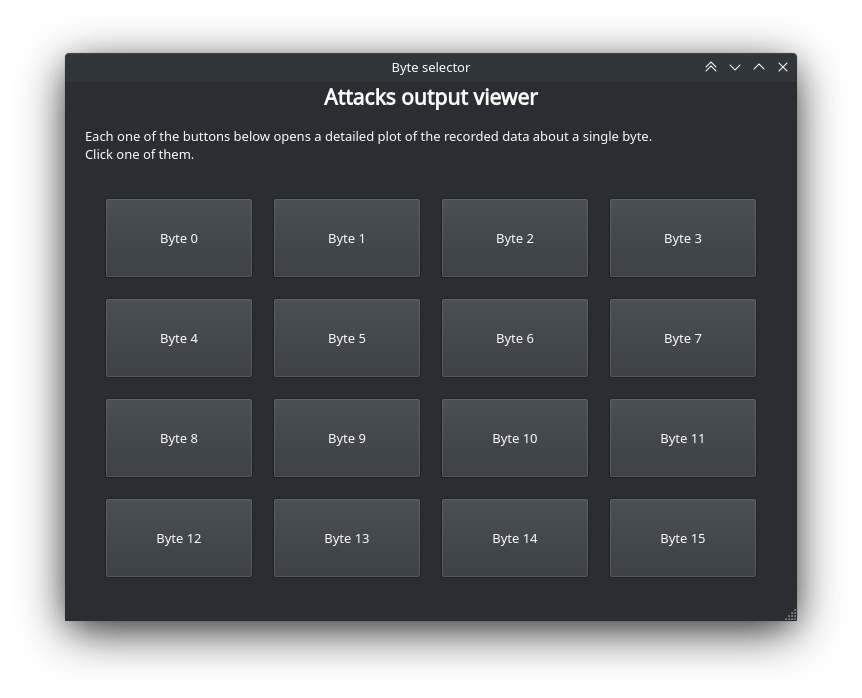
\includegraphics[scale=0.6]{main_window.png}
    \caption{Main window of the program.}
    \label{fig:main_window}
\end{figure}

\subsection{Nice to have improvements}
Some safety measures have been implemented to guarantee the right course of action of the application.
Our implementation makes an extensive use of files I/O, both for reading and writing data.
If, by any chance, one of the file is not placed in the correct directory or not present at all, an error message will be printed to the console and the script will terminate.
Also, some correlation values in the files might be corrupted or not available (i.e., NaN values).
The preprocessing scripts check for that and replace them with null values (i.e, zero).
An error will be also thrown if those two scripts are not run or run in the wrong order.

%-----------------------------------------------------------------------------
% ENCOUNTERED PROBLEMS AND SOLUTIONS
%-----------------------------------------------------------------------------

\section{Faced problems and solutions}
\label{sec:faced-problems-and-solutions}

During the development of the application, we had to face up some problems, mainly due to the size of the dataset to handle.
We think it can be useful to share here some insights about our decision-making process as the developement was moving forward, and the solutions we came up with.

\subsection{The starting point}

Starting from the very beginning, our goal was plotting the content of a \texttt{.csv} file, while maintaing the possibility of moving around inside the plot (i.e., zoom-in, zoom-out, change the X-range).\\

Our initial approach was plotting all the file at once.
The problem that immediately arised was that handling over 7.5 million points (every \texttt{.csv} file has about 35 thousand rows and 256 columns) was definitely too resource-demanding.
That led to an evidently unusable GUI due to its poor performance, not only when moving around, but also for the loading time of the plot itself.\\

Therefore, we started looking for some possible improvements on how to load data into memory in an efficient way using Python.\\

\subsection{Choosing the fastest file format}

A first available option we found was converting the \texttt{.csv} file into a \texttt{.hdf5} one.
\texttt{HDF5} is a file format built for fast I/O processing and storage, whose potential can be fully exploited through a handy Python library.

However, the result we obtained was still very poor and the \texttt{HDF5} option had to be discarded.\\

Since we handled all the data as \texttt{NumPy} arrays, we also came across the \texttt{.npy} file format.
It is a simple format for saving \texttt{NumPy} arrays, in an optimized way, with no loss of information.
After converting the \texttt{.csv} file into a \texttt{.npy} one, we plotted it in the same way as before.
The loading time was significantly lower and the usability of the GUI improved, but still far from an acceptable result.\\

\subsection{Downsampling}

Having understood that \texttt{.npy} was a far better choice over \texttt{.csv} and \texttt{.hdf5}, we decided to keep that conversion step and start tweaking around to gain as much performance as possible, this time in the \texttt{PyQtGraph} plotting process.

A special tweak we would like to highlight is the way we subsample data in order to display it in the plot.
\texttt{PyQtGraph} provides three downsampling modes: subsample, mean, and peak.

Despite being the slowest one, we picked the last one ("peak") since it downsamples by drawing a saw wave that follows the min and max of the original data.
This is the only way to make sure that the peak of our plot does not get lost while displaying the points.\\

\subsection{Plotting one curve at a time}

Back to the fact that the GUI responsiveness was far from being acceptable, we came to the conclusion that showing all the 7.5 M points at the same time was not feasible in any way.

At this point we tried to change our approach. Here was (and currently is) our new one.

Since every file contains 256 rows, and each row corresponds to a curve in the plot, we can preprocess every file and identify for it which is the peak and what row it shows up in. Then, save these results in a new file.
When the user opens a plot, the program can read the content of that new file to display by default only the curve with the peak.
In addition, each one of the other curves can be shown/hidden in the plot by using a dedicated checkbox on the right side of the window.\\

This new approach leads to a very low loading time and to a GUI which is not only usable, but also high-performing in every zoom/scroll operation.\\

Despite the noticeable performance increase intrinsic to the new way of displaying data, we still decided to keep the conversion step from \texttt{.csv} to \texttt{.npy}.
In fact, the same file stored as \texttt{.npy} takes more than 40\% less space on disk than if stored as \texttt{.csv}.
As we will cover in more detail in the next section, this leads to both faster loading times and lower memory usage at runtime.

\begin{figure}[H]
    \centering
    \subfloat[Showing only the curve with the peak.\label{fig:single_curve}]{
        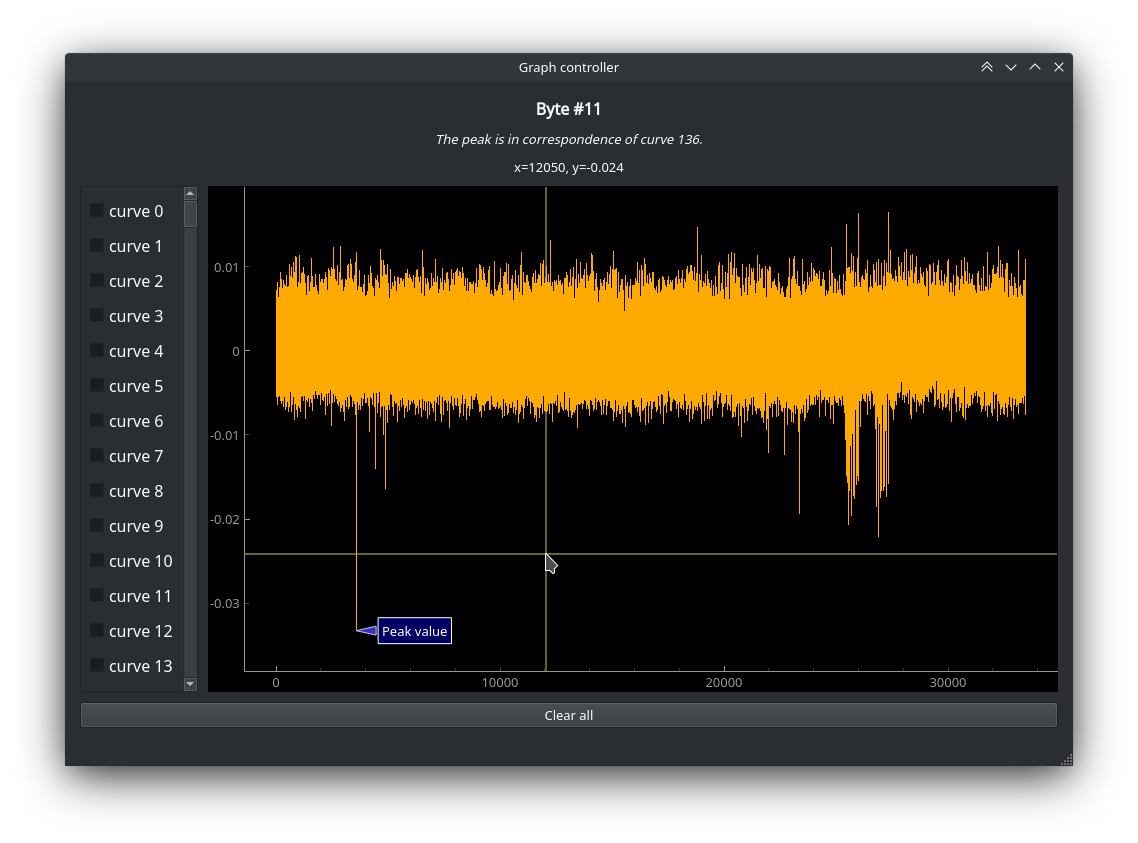
\includegraphics[width=0.95\textwidth]{img/single_curve.png}
    }
    \quad
    \subfloat[Showing multiple curves.\label{fig:multiple_curves}]{
        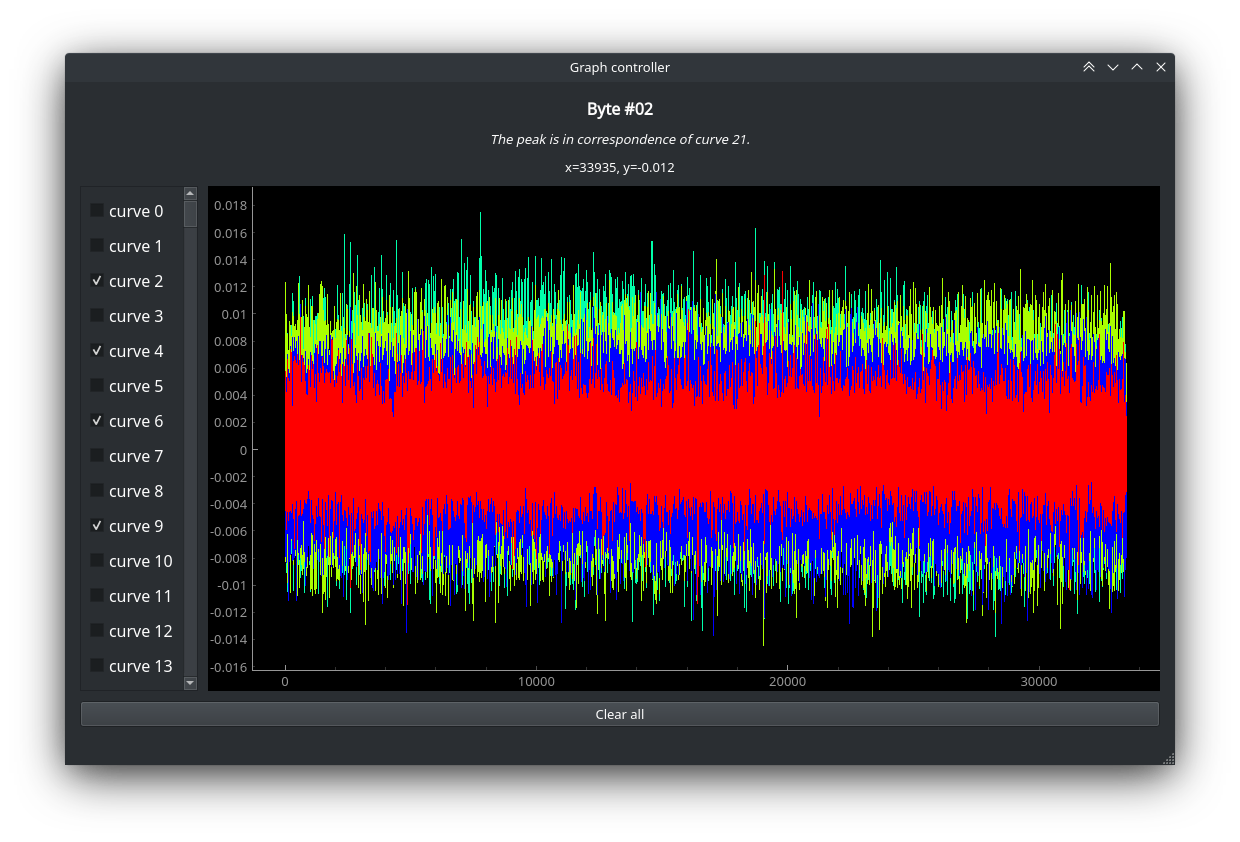
\includegraphics[width=0.95\textwidth]{img/multiple_curves.png}
    }
    \caption[]{Examples of two plots created with \texttt{PyQtGraph}.}
    \label{fig:plots}
\end{figure}

%-----------------------------------------------------------------------------
% EXPERIMENTAL RESULTS
%-----------------------------------------------------------------------------

\section{Experimental results}
\label{sec:experimental-results}

Here are some useful measurements about execution time and memory usage of the program.

\subsection{Testing conditions}

All the tests have been performed on a machine with an i7-7500U CPU (dual-core @ 2.70 GHz) and 8 GB of RAM.
Keep in mind that the execution time will vary from machine to machine.
Since at the moment of writing the hardware above can be considered mid/low-end, you can likely expect better results when running the scripts.\\

The 16 \texttt{.csv} input files have each one 256 columns and about 30 thousand rows.

\subsection{Conversion from .csv to .npy}

The preprocessing step of converting the 16 files to the \texttt{.npy} format is performed by the \texttt{csv\_to\_npy\_converter.py} script.
It runs for 2m00s while using 1.1 GB of memory (maximum instant value recorded, in average it takes up less memory).

\subsection{Peak detection}

The preprocessing step of detecting the peak value of each one of the files is performed by the \texttt{peak\_detection.py} script.
When the \texttt{--save-png} flag is used, in addition to detecting the peaks it also generates and saves the plots of all the files.
In such a case the total execution time is 1m55s, with a memory consumption of 550 MB at its highest point.

However, by default the plots are not generated and this way the execution time is extremely reduced: it goes down to just 1s.

\begin{figure}[H]
    \centering
    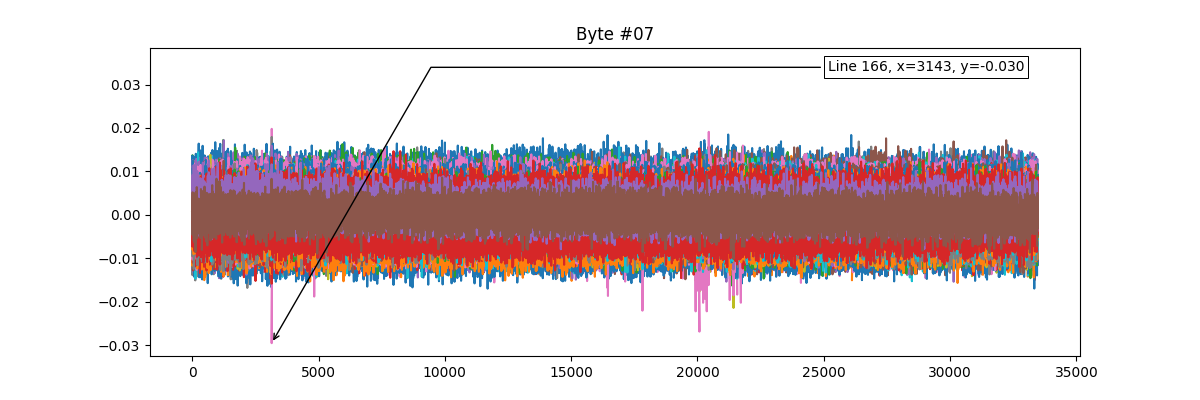
\includegraphics[scale=0.55]{static_plot.png}
    \caption{Static plot generated by \texttt{peak\_detection.py}.}
    \label{fig:static_plot}
\end{figure}

\subsection{Main program}

For the main program (\texttt{main.py}), we recorded the change in memory consumption by varying the number of open plots and displayed curves.\\

In particular, the obtained results in memory consumption are the following (rounded up values are reported):
\begin{itemize}
    \item the main window uses 125 MB;
    \item every other window uses:
    \begin{itemize}
    		\item 65 MB for loading the .npy file (which is the size on disk of the file);
    		\item 5 MB for the creation of the window;
    		\item 1 MB for every displayed curve.
	\end{itemize}
\end{itemize}

%-----------------------------------------------------------------------------
% CONCLUSIONS
%-----------------------------------------------------------------------------

\section{Conclusions}
\label{sec:conclusions}

This report shows the implementation of a data visualization tool mainly based on \texttt{PyQt} and \texttt{PyQtGraph}.
An effort was made to make the user experience smooth and efficient, even though the amount of data is very high.
Some of the encountered issues were discussed and the chosen solutions were presented.\\

We hope that this tool can be a useful basis for some future work targeting an even more efficient implementation.
Given the many capabilities that \texttt{PyQtGraph} has, there is plenty of room for adding features and expanding the application.\\

As a final note,  keep this in mind: in case you will have to deal with much larger datasets and you want to see the results as soon as possible, a good approach could be plotting directly the .csv files.
In fact, you will remove the preprocessing step of converting files to .npy (even if you just need to run it once), thus gaining some minutes at the expense of a larger memory footprint and a worse runtime performance.

In every case, remember that it is always about tradeoffs.

%-------------------------------------------------------------------------
%	END OF YOUR DOCUMENT
%-------------------------------------------------------------------------

\end{document}
